%-------------------------
%minimal-unix
%(c) H.Buchmann FHNW 2017
%export TEXINPUTS=.:${HOME}/fhnw/edu/:${HOME}/fhnw/edu/tinL/config/latex:${HOME}/fhnw/edu/config//:
%-------------------------
\documentclass{beamer}
\usepackage{latex/beamer}
%---------------------
%local defines
%(c) H.Buchmann FHNW 2009
%$Id$
%---------------------
\newcommand{\target} {\beaglebone\xspace}
\newcommand{\targetS}{{\bf BBG}\xspace}
\newcommand{\host}   {{\em Host}\xspace}
\newcommand{\targetroot} {{\bf target-root}\xspace}
\newcommand{\kernel} {{\bf kernel}\xspace}
\renewcommand{\c}{{\bf C}\xspace}
\newcommand{\cpp}{{\bf C++}\xspace}
\newcommand{\posix}{{\bf POSIX}\xspace}

\input{/home/buchmann/latex/dirtree/dirtree.tex}

\usepackage[absolute]{textpos}
\setlength{\TPHorizModule}{1mm}
\setlength{\TPVertModule}{1mm}

\begin{document}

\newcommand{\md}{\cod{md-bbb-{\em version}.img}}
\newcommand{\mdev}{\cod{md-bbb-devel-{\em version}.tar.gz}}
\title{�berblick}

\frame{\titlepage}

\begin{frame}{Die Herstellung von einem \linux}{eine komplexe Angelegenheit}
 \begin{block}{Gegegben}
  \begin{itemize}
   \item Files von �berall her  
   \begin{itemize}
    \item meistens Sourcefiles
   \end{itemize}
  \end{itemize}
 \end{block}
 \begin{block}{Gesucht}
  \begin{itemize}
   \item \linux, \unix
   \begin{itemize}
    \item Betriebssystem
   \end{itemize}
  \end{itemize}
 \end{block}
\end{frame}

\begin{frame}{Betriebssystem}{Sammlung von Programmen auf einem Rechner}
  \begin{itemize}
   \item wenig-viele Programme
   \item kleiner-grosser Rechner
  \end{itemize}
\end{frame}

\begin{frame}{Unser Betriebssystem und Rechner} 
 \begin{itemize}
  \item Target 
  \begin{itemize}
   \item \target
   \item \linux eher klein
  \end{itemize}
  \item \host
  \begin{itemize}
   \item \unix eher gross
  \end{itemize}
 \end{itemize}
\end{frame}

\section{\target}
\begin{frame}{\target}{Was haben wir ?}
 \begin{itemize}
  \item Hardware mit WLAN
  \item Debian im Flash
  \item SD-Card Fassung
  \begin{itemize}
   \item f�r eigenes \linux
  \end{itemize}
  \item \cod{doc/beaglebone-black/BBB\_SRM.pdf}
 \end{itemize}
\end{frame}

\section{Debian}
\begin{frame}{Debian:Verbindungen}{Siehe \cod{3-network}}
  \begin{itemize}
   \item USB/Internet
   \item WLAN/Internet
   \item \cod{ssh} Secure Shell 
   \item \target - WAN
  \end{itemize}
\end{frame}


\section{From Scratch}
\begin{frame}{\linux:von Grund auf}{Image auf SD-Karte}
 \begin{itemize}
  \item Bootloader
  \item Kernel
  \item RootFS
 \end{itemize}
\end{frame}

\begin{frame}{The Big Picture}
\begin{center}
 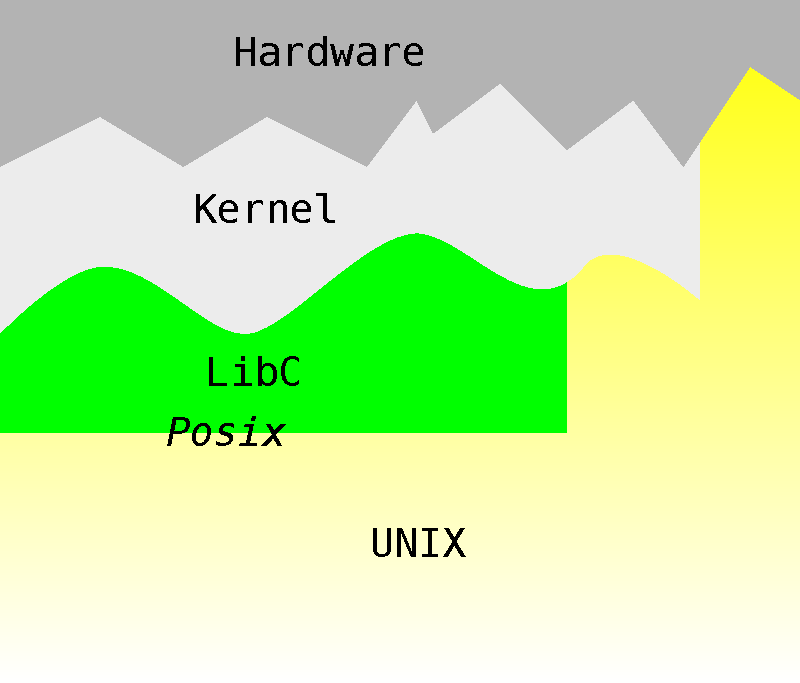
\includegraphics[height=0.875\textheight]{layers.pdf}
\end{center}
\end{frame}

\subsection{Partitionen}
\begin{frame}{Image: 2 Partitionen}{Siehe \cod{3.5-partitions}}
 \begin{description}[Partition 1: p1]
  \item[Partition 1: p1] \cod{vfat} Bootloader, kernel 
  \item[Partition 2: p2] \cod{ext4} RootFS
  \item[Befehle] auf dem \host
  \begin{itemize}
   \item \cod{fdisk} 
   \item \cod{mkfs.vfat}
   \item \cod{mkfs.ext4}
  \end{itemize}
 \end{description}
\end{frame}

\subsection{Boot/Kernel}
\begin{frame}{Herstellung}{Teil 1: wenig files}
 \begin{description}[toolchain-bare:]
  \item[toolchain-bare:] Siehe \cod{17-build/tools/\{binutils.sh | gcc-bare.sh\}}
  \item[u-boot:] Siehe \cod{4-uboot}
  \begin{itemize}
   \item \cod{MLO}
   \item \cod{u-boot.img}
  \end{itemize}
  \item[kernel:] Siehe \cod{5-kernel}
  \begin{itemize}
   \item \cod{zImage}
   \item \cod{am335x-boneblack-wireless.dtb}
  \end{itemize}
 \end{description}
\end{frame}

\newcommand{\targetRoot}[1]
{
{
\footnotesize
\setlength{\DTbaselineskip}{0.875em}
\dirtree{%
.1 #1.
.2 bin.
.2 dev.
.2 etc.
.2 home.
.2 lib.
.2 linuxrc.
.2 made-{\em yyyy-mm-dd}.
.2 proc.
.2 sbin.
.2 share.
.2 sys.
.2 usr.
}
}
}

\subsection{RootFS}
\begin{frame}{Herstellung RootFS}{\host\ - SD-Card - Target(\targetS)}
\begin{columns}
\begin{column}{0.3\textwidth}
 \host
 
 \targetRoot{{\em path-to-target-root}}
\end{column}
\begin{column}{0.3\textwidth}
 SD-Card
 
 \targetRoot{{\em path-to-sd-card}}
\end{column}
\begin{column}{0.3\textwidth}
 \targetS
 
 \targetRoot{/}
\end{column}
\end{columns}
\begin{block}{Transport}
 \vspace{-2mm}
 \begin{description}[SD-Card $\to$ \targetS:]
  \item[\host $\to$ SD-Card:] \cod{rsync -av {\em path-to-target-root} {\em path-to-sd-card}}
  \item[SD-Card $\to$ \targetS:] einstecken
  \item[SD-Card $\to$  \host:]\cod{rsync -av {\em path-to-sd-card} {\em path-to-target-root}}
 \end{description}
\end{block}
\end{frame}


\begin{frame}{Herstellung}{Teil 2: RootFS}
 \begin{description}[toolchain] 
  \item[LibC] Siehe \cod{17-build/tools/glibc.sh}
  \item[toolchain] \cod{17-build/tools/gcc.sh}
  \item[\unix] Verschiedene {\em flavours}
  \begin{itemize}
   \item minimal: Siehe \cod{19-minimal}
   \item busybox: Siehe \cod{17-build/tools/busybox.sh}
  \end{itemize}
 \end{description}
\end{frame}

\begin{frame}{Ausbau}
 \begin{description}[WLAN]
  \item[ssh]  Siehe \cod{17-build/tools/openssh.sh}
  \item[WLAN] Siehe \cod{6-assembly}
  \item[init] Siehe \cod{6-assembly}
 \end{description}
\end{frame}


\section{Aufgaben}

\begin{frame}{Ziel}
 \begin{itemize}
  \item \cod{hello-world} auf dem \host und auf dem \targetS
  \item \cod{primes} auf dem \host und auf dem \targetS
 \end{itemize}
\end{frame}


\begin{frame}{The big Picture}
 \begin{itemize}
  \item Source File: \cod{hello-world.cc}
  \item falls es nicht klapt ?
  \begin{itemize}
   \item wo ist der File ?
  \end{itemize}
 \end{itemize}
\end{frame}


%\subsection{Die Programme}
%\begin{frame}{Development}{\cod{hello-world-c.c}}
%\hspace*{-8mm}
%{
%\begin{tabular}{llllll}
% Host & Target & OS & Toolchain & Verbindung & Bemerkungen\\
% \hline
% \targetS & \targetS & Debian & mitgeliefert&&\\
% \host   & \targetS & Debian & \cod{\tiny tc-tinl-gcc-8.1.0-2018.05.21.tar.gz} & sshfs\\
% \host   & \targetS & minimal & \cod{\tiny tc-tinl-gcc-8.1.0-2018.05.21.tar.gz} & SD-Card  &später\\
% \host   & \targetS & minimal & \cod{\tiny tc-tinl-gcc-8.1.0-2018.05.21.tar.gz} & curlftpfs&später\\
%\end{tabular}
%}
%\remark{Toolchain auf der Cloud: \href{https://drive.switch.ch/index.php/s/A6H382zEGDrgfAL}
%       {\Huge tinL}}
%\end{frame}

\end{document}
